\\

A short introduction to sEMG was given in the control systems section \ref{sEMG}. A more detailed description on how to make input control system from the sEMG can be found later in the report.

\paragraph{Electromyography} or EMG. as it has been called throughout this project, is a visualisation of the sum of difference in the potential measured fibres within one muscle. A skeletal muscle is made up of many small fibres called myofibril that each produces a difference in the potential. This signal needs amplification furthermore the signal has to be processed with the help of the analogue process, as described later in the section, in order to create a reliable source of control. The use of EMG is well documented in different articles in the use of a prosthetic arm  \cite{Castellini2009}. The EMG signal in this report is used to describe the signal that is being interpret.

\subsection*{Signal processing}
When the control unit receives the sEMG data, either through a micro-controller or a computer that processes the data, the data is the raw input data from the sEMG and cannot be used as an input for a control system. It is therefore clear that there is a need for processing the received data. In this project the signal is analysed through method of root mean square(RMS) which is an implemented part of the hardware, this is described later in this section.
\\ 

\subsubsection{Filters}
Digital filters is an important part of signal processing. 
These filters removes the noise in the signal depending on what frequencies of the signal that is useful for a robot or radio. A robot needs low frequencies due to it being a mechanical system.\\
Filters are classified as the frequency types it will filter on the signal. Two of the filters, the \textbf{low-pass} and the \textbf{high-pass} describes the filters that let the signal pass above or below a certain cutoff frequency. There is also the band-pass, and the band-stop filter which let the frequency's in a defined bandwidth pass through or block them respectively.
The most suited filter should be chosen based on analysis of the signal.

\paragraph{Sampling}
Certain precautions needs to be taken when sampling the sEMG signal. according to the \textit{Nyquist theorem} the sampling rate should be at least twice that of the signal frequency in order to insure the sinusoid of the EMG signal can be recreated. If this is not done then the data could be corrupted by the aliasing phenomenon. \cite{Nyquist}

%there are in general two use categorys, \textit{signal separation} and \textit{signal restoration}. \cite{FilterBa67:online}


%\paragraph{Signal separation} as the name implies this category seperates the signal passed through. this is normally used when the signal is contaminated with signal noise or other interference. in praxis an example could be a muscle sensor on the pectoralis major. here the signal might be contaminated with noise from the heart or other muscles. 
%therefore there would be a need to seperate the signals and isolate the wanted muscle signal.\cite{FilterBa67:online}
%\paragraph{signal restoration} this refers to when a signal has been distorted. an example could be an audio recording. after filtering it, the sound quality might improve beyond the original. \cite{FilterBa67:online}

\subsection*{Electronic hardware} \label{sec:elHW}
For a signal to be used in a software application there is a need for a way to interpret the signal. In this project the use of an EMG signal requires a hardware part, in this case, it is the muscle sensor v 3.0 from Advancer technology. The muscle sensor measures the signal through the electrodes placed on the user, furthermore, the device amplifies the signal by a gain of 100, it also rectifies the wave signal, which will be described later. The EMG sensor smooths the signal and convert it from an analogue signal to a digital signal that can be processed\cite{EMGHARD}.\\
As seen in figure: \ref{fig:GainsEMG}, the gain is decided through resistor R1, the voltage goes through MID and END, which are EMG inputs. The EMG signals then get amplified across the operational amplifier(OP AMP).\\

\begin{multicols}{2}  
\begin{figure}[H]
    \centering
    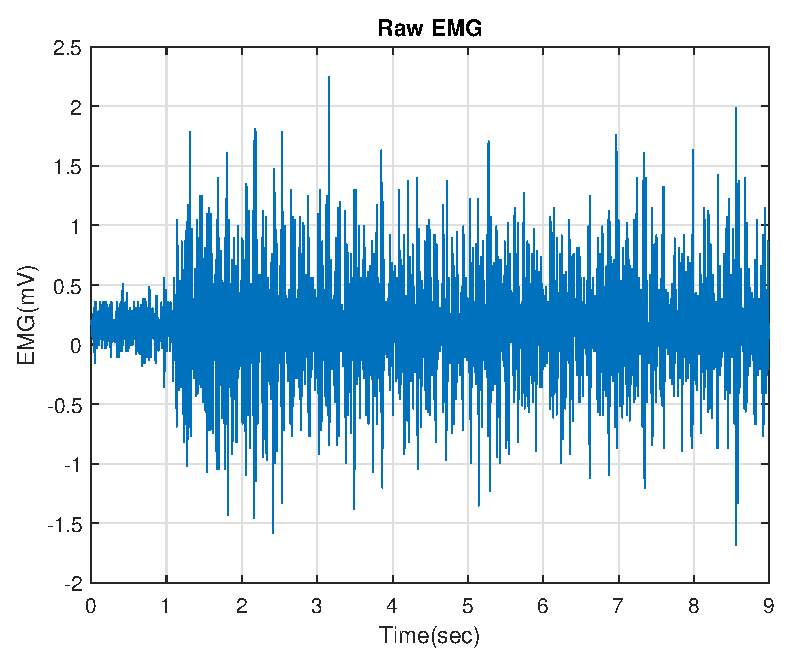
\includegraphics[width=0.4\textwidth]{Figures/EMG/epsFigRAW}
    \caption{\centering{EMG in a raw form analysed \\through matlab, data was borrow from\cite{EMGDATA}}}
\end{figure} 
\columnbreak
\begin{figure}[H]
    \centering
    \includegraphics[width=0.4\textwidth]{Figures/EMG/AmpGB.PNG}
    \caption{\centering{The schematics of the gain of the sEMG signal}\cite{SparkfunScematicEMG}}
    \label{fig:GainsEMG}
\end{figure} 
\end{multicols}

\paragraph{Full wave}
rectifying can be done by hardware or software. The software approach can be done simply by taking the absolute value  of the input data, in this case the hardware rectify the wave\cite{RMS}. Since the signal is an alternating waveform the signal is now only represented as positive numbers. Furthermore, the negative part of the data-set is conserved by squaring the value. This is important for the next step in analysing the data signal, and the root mean square process.\\
The schematics of rectifying the signal can be seen in \ref{fig:rect}, has a input from the latest schematic "Measure", where it polarises the input through a capacitor, and send the polarised signal through a 150k resistor. The signal is then sent through a serial connection, connected with junctions which includes known OP AMP's and ground inputs. The signal is now rectified.\\

\begin{multicols}{2}
\begin{figure}[H]
    \centering
   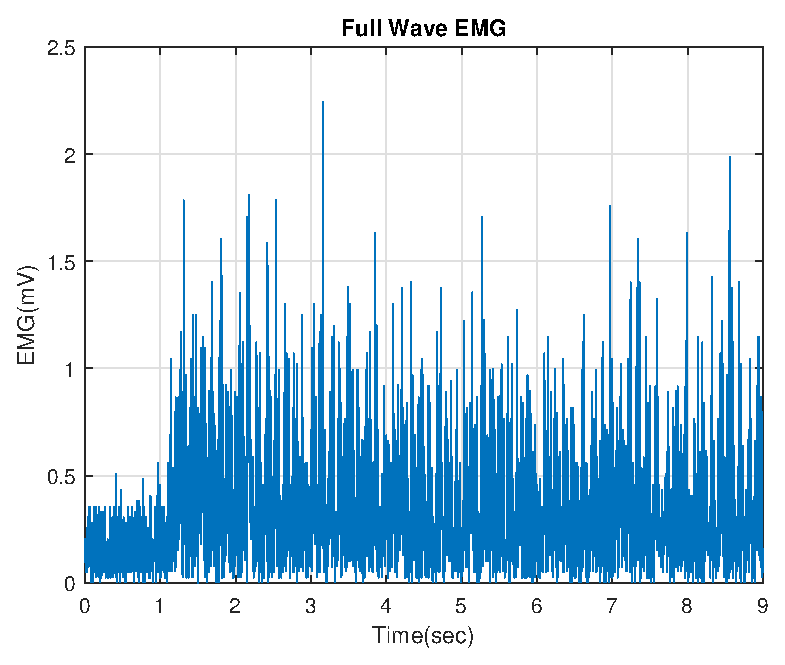
\includegraphics[width=0.3\textwidth]{Figures/EMG/epsFig}
    \caption{\centering{ EMG in Full wave form analysed \\through Matlab, data was borrow from \cite{EMGDATA}}}
\end{figure} 
\columnbreak
\begin{figure}[H]
    \centering
    \includegraphics[width=0.7\textwidth]{Figures/EMG/Rect.PNG}
    \caption{\centering{The schematics of the rectifying on the EMG sensors}\cite{SparkfunScematicEMG}}
    \label{fig:rect}
\end{figure} 
\end{multicols} 
\paragraph{Root mean square} or RMS is a solution made in order to get an average over time from any signal. It needs the wave form described in the full wave, this is referring to the squared part of RMS, so the means of the EMG signal can be evaluated, refraining from the rectifying of the squared part gets the mean of zero\cite{RMS}. After processing the signal it
is used as an implementation for a control signal.\\
The next step of schematics is as seen in \ref{fig:smooth}, is smoothing out the signal as described above. The rectified signal gets processed in a serial connection with known OP AMP's, resistors and capacitors. When the EMG signal is sent through this part of EMG sensor, the signal is smoothed.\\
The last schematics \ref{fig:finalGain}, with smooth signal as input, it is again put through a OP AMP to get the last gain before the signal is converted into a digital representation of the signal. The gain in this OP AMP is decided through the potentiometer.\\


\begin{multicols}{2}
\begin{figure}[H]
    \centering
    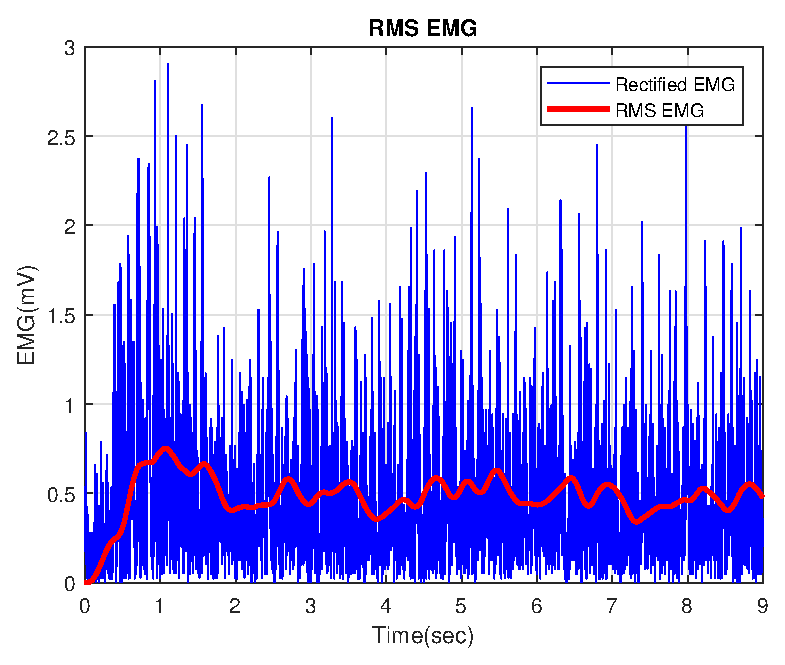
\includegraphics[width=0.4\textwidth]{Figures/EMG/epsFigRMS}
    \caption{EMG in Full wave with RMS analyses\\ preformed in matlab, data was borrow from\cite{EMGDATA}}
    \label{ref:Wasmooth}
\end{figure}
\columnbreak
\begin{figure}[H]
    \centering
    \includegraphics[width=0.4\textwidth]{Figures/EMG/Smooth.PNG}
    \caption{The schematics of the smoothing on the EMG sensors\cite{SparkfunScematicEMG}}
    \label{fig:smooth}
\end{figure} 
\end{multicols}




\begin{figure}[H]
    \centering
    \includegraphics[width=0.5\textwidth]{Figures/EMG/FinalGain.PNG}
    \caption{\centering{The schematics of the last gain on the EMG sensors before data is transmitted\cite{SparkfunScematicEMG}}}
    \label{fig:finalGain}
\end{figure} 


\subsection*{Muscle choice}
 Any distinct muscles which can voluntarily be controlled by the user could, in theory, be used as the input to the control system. Examples of possible choices could be the use of facial muscles, or the use of the muscles from the remaining arm. Surgically attaching the muscles closer to the skin to get a better signal is also an option \cite{SimonsSu49:online}.\\
 Difficulties in receiving a stable signal will change depending on the electrodes location on the body, e.g the breast muscles on the upper torso. The torso-muscles could be an ideal choice for some users, but if the electrodes were to be placed close to the heart, the heart-rhythm could interfere with the signal, while heightening the difficulties in receiving a stable control signal, due to the added noise from the heart, and would need to be filtered out. \\
 As a proof of concept the muscles in the lower arm as seen in figures \ref{ref:UpperArm} and \ref{fig:UnderArm} is used due to their accessible location when placing the electrodes while testing.
\begin{multicols}{2}
\begin{figure}[H]
    \centering
    \includegraphics[width=0.4\textwidth]{Figures/Technical_figures/OverArm.jpg}
    \caption{Picture showing the placement of electrodes on top of the forearm, where the green electrode is the neutral point, and both the black and red electrodes are placed on the same muscle}
    \label{ref:UpperArm}
\end{figure}
\columnbreak
\begin{figure}[H]
    \centering
    \includegraphics[width=0.4\textwidth]{Figures/Technical_figures/UnderArm.jpg}
    \caption{Figure showing the placement of electrodes under the forearm, where green is the neutral point, and both black and red is on the same muscle}
    \label{fig:UnderArm}
\end{figure} 
\end{multicols}